\documentclass[a4paper,12pt]{article} 

%%% Работа с русским языком
\usepackage{cmap}                           % поиск в PDF
\usepackage{mathtext} 			 	       % русские буквы в формулах
\usepackage[T2A]{fontenc}               % кодировка
\usepackage[utf8]{inputenc}              % кодировка исходного текста
\usepackage[english,russian]{babel}  % локализация и переносы
\usepackage[left=2cm,right=2cm,
    top=2cm,bottom=3cm,bindingoffset=0cm]{geometry}
\usepackage{wrapfig}
\usepackage{gensymb}
\usepackage{textcomp}
\usepackage{multirow}
\usepackage{pgfplots}
\usepackage{amsmath,amsfonts,amssymb,amsthm,mathtools} % AMS
\usepackage{euscript}	 % Шрифт Евклид
\usepackage{mathrsfs} % Красивый матшрифт
\usepackage{graphicx}%Вставка картинок правильная
\usepackage{float}%"Плавающие" картинки
\usepackage{wrapfig}%Обтекание фигур (таблиц, картинок и прочего)
\title{Лабораторная работа 4.3.4

Метод преобразования Фурье в оптике}
\author{Кагарманов Радмир Б01-106}
\date{10 мая 2023 г.}

\begin{document}
\maketitle
\thispagestyle{empty}
\newpage
\setcounter{page}{1}

\paragraph*{Цель работы:} Исследовать явления дифракции Френеля и Фраунгофера на щели, изучить влияние дифракции на разрешающую способность оптических приборов.
\paragraph*{В работе используются:} Гелий-неоновый лазер, кассета с набором
сеток разного периода, щель с микрометрическим винтом, линзы,
экран, линейка.
$$$$
Анализ сложного волнового поля во многих случаях целесообразно проводить, разлагая его на простейшие составляющие, например, представляя его в виде разложения по плоским волнам. При этом оказывается, что если мы рассматриваем поле, полученное после прохождения плоской монохроматической волны через предмет или транспарант (изображение предмета на фотоплёнке или стеклянной пластинке) с функцией пропускания t(x), то разложение по плоским волнам соответствует преобразованию Фурье от этой функции. Если за предметом поставить линзу, то каждая плоская волна сфокусируется в свою точку в задней фокальной плоскости линзы. Таким образом, картина, наблюдаемая в фокальной плоскости линзы, даёт нам представление о спектре плоских волн падающего на линзу волнового поля. Поэтому можно утверждать, что с помощью линзы в оптике осуществляется пространственное преобразование Фурье.

\section*{Определение ширины щели}
\label{section_I}
\subsection*{Экспериментальная установка}

Схема установки представлена на рис. \ref{fig:scheme_I}. Щель переменной ширины D, снабжённая микрометрическим винтом В, освещается параллельным пучком света, излучаемым лазером (радиус кривизны фронта волны велик по сравнению с фокусными расстояниями используемых в схеме линз).

\begin{figure}[h]
    \centering
    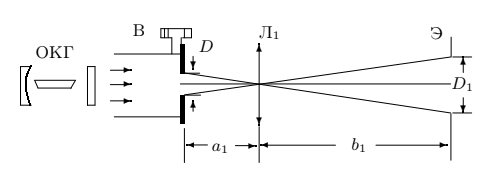
\includegraphics[width=15cm]{scheme_I.png}
    \caption{Схема лабораторной установки для определения ширины щели}
    \label{fig:scheme_I}
\end{figure}

Увеличенное изображение щели с помощью линзы Л1 проецируется на экран Э. Величина изображения D1 зависит от расстояний от линзы до предмета — $a_1$ и до изображения — $b_1$, т. е. от увеличения $\Gamma$ системы:

$$\Gamma=\frac{D_{1}}{D}=\frac{b_{1}}{a_{1}}$$

\newpage

\subsection*{Измерения}

\begin{enumerate}
    \item Соберем схему с Рис. \ref{fig:scheme_I}, используя короткофокусную линзу $F_3 = 4.3$ см.
    \item Определим начало открытия щели: $pos_0 = 0.68$ мм
    \item Меняя ширину щели от 50 до 500 мкм (5–50 делений от нового нуля), снимем зависимость размера изображения $D1$ от ширины щели $b$. Построим график этой зависимости.
\begin{figure}[!h]
\centering
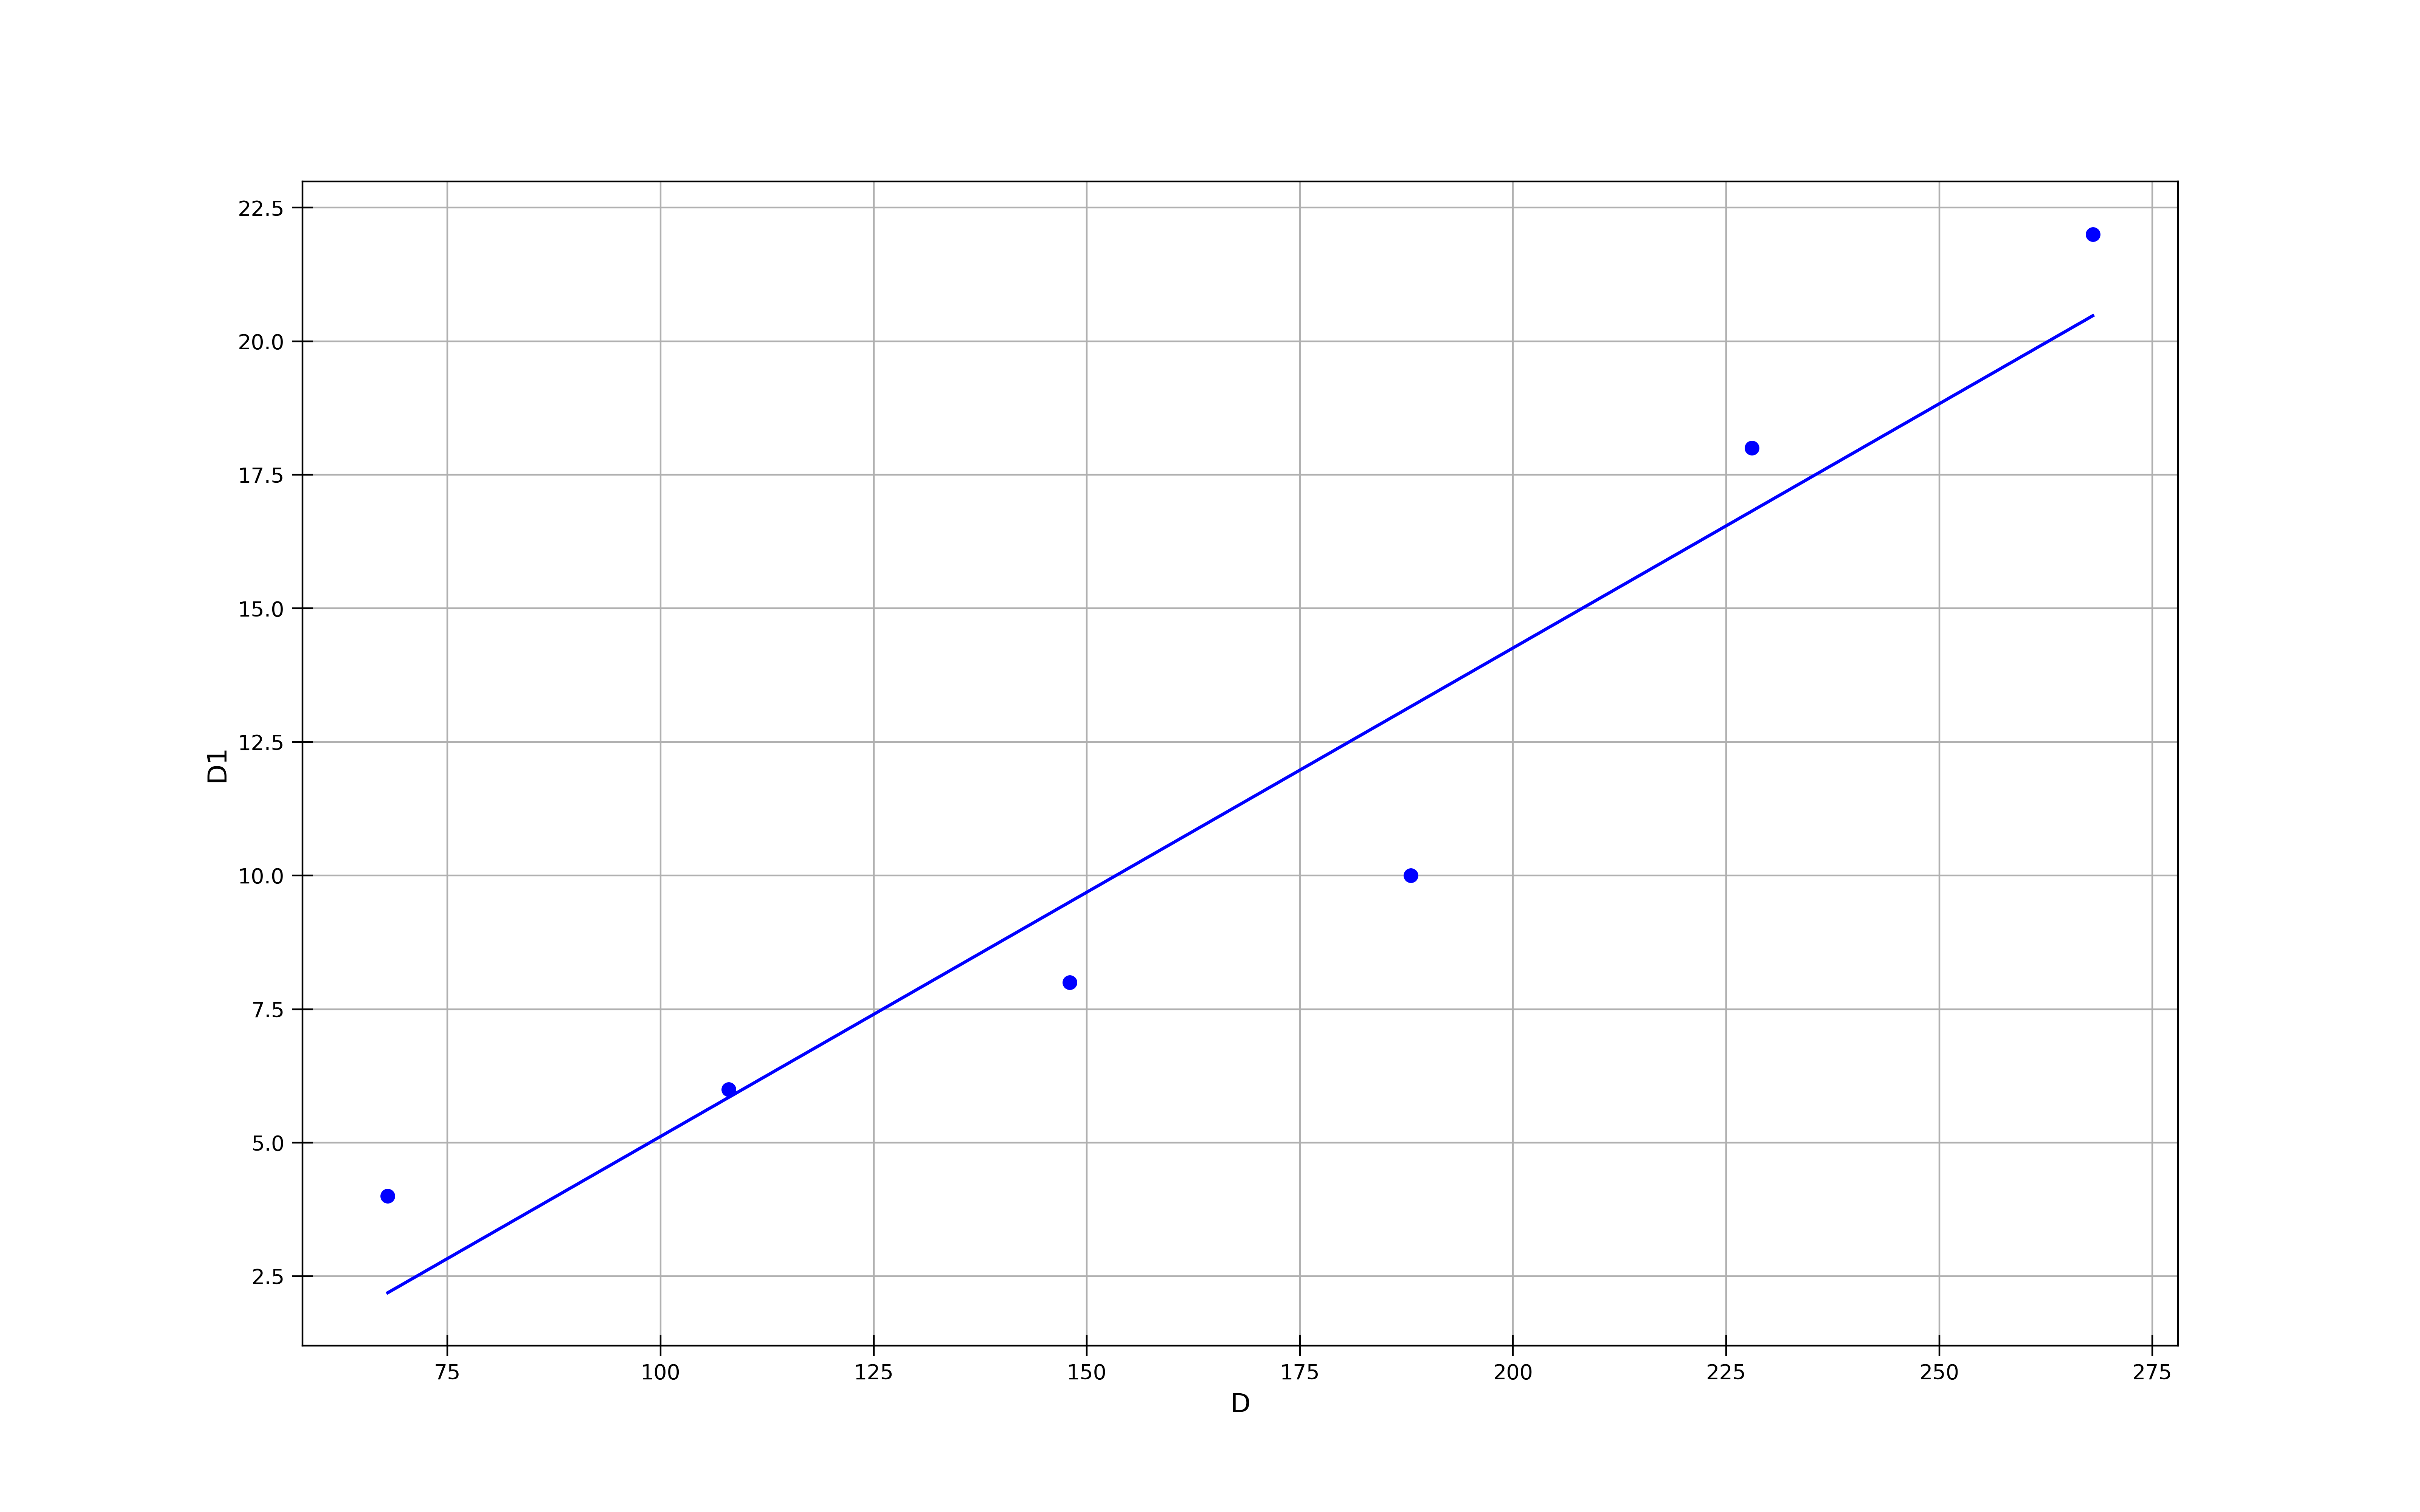
\includegraphics[width=0.9\linewidth]{f1.png}
\caption{Зависимость D1 от D}
\label{fig:mpr}
\end{figure}

    \item Измерим расстояния $a_1 = 45 \pm 1$ мм и $b_1 = 1325 \pm 1$ см. По ним вычислим $\Gamma = 29.4 \pm 0.6$.
    По графику найдем точный момент открытия щели $b = 0.45мм$.
\end{enumerate}

\section*{Определение ширины щели по её спектру}

\subsection*{Экспериментальная установка}

Убрав линзу, можно наблюдать на экране спектр щели (рис. \ref{fig:scheme_II})

\begin{figure}[h]
    \centering
    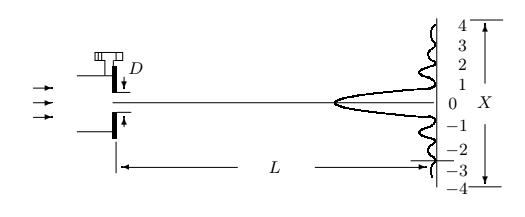
\includegraphics[width=15cm]{scheme_II.png}
    \caption{Спектр щели}
    \label{fig:scheme_II}
\end{figure}

\newpage

\subsection*{Измерения}

\begin{enumerate}
    \item Получим на удалённом экране спектр щели (рис. \ref{fig:scheme_II}). Меняя ширину щели проследим за изменением спектра на экране и оценим интервал, для которого можно наблюдать и измерять спектр.
    \item Проведем измерения ширины $m$ минимумов (центральный считается за 2) для диапазона такого диапазона ширины, как в пункте I. Занасем результаты в Таблицу 2. ($b$ в этой части отмеряется от $b_0 = 0.42$ мм)
    
   
    
    По графику найдем точный момент открытия щели $b_{II} = 0.61мм$ и угловой коэффициент $k = 1.4$ 1/$\text{мм}^2$ $\approx \frac{1}{\lambda L} = 1.26$ 1/$\text{мм}^2$, измерив $L = 125$ см.
    
\end{enumerate}

\section*{Определение периода решёток}

\begin{enumerate}
    \itemПоставим кассету с двумерными решётками (сетками) вплотную к выходному окну лазера. Для каждой сетки измерим расстояние $X$ между $m$-ми пиками и отметим $m$ — количество пиков. Рассчитаем расстояния $\Delta X$ между соседними максимумами и определим период каждой решётки $d_с = f(\Delta X)$, используя соотношения:
        \begin{equation*}
            \Delta X=\frac{X}{m}=\frac{\lambda}{d_{\mathrm{c}}} L
        \end{equation*}
        Результаты занесем в Таблицу \ref{table::no_lenses}.
    
        \itemДалее линзу Л$_{2}$ с максимальным фокусом $\left(F_{2} = 11 \mathrm{~cm}\right)$ поставим на расстоянии $\simeq F_{2}$ от кассеты. В плоскости Ф линза Л$_{2}$ даёт Фурье-образ - сетки её спектр, а короткофокусная линза Л$_{3}\left(F_{3} = 2,5 \mathrm{~cm}\right)$ создаёт на экране увеличенное изображение этого спектра (Рис \ref{fig:scheme_III}).
        Измерим $X$ и $m$ для всех сеток, где это возможно. Так как экран достаточно удалён $\left(b_{3} \gg a_{3}\right)$, то практически $a_{3}=F_{3}$, и расстояние между линзами $\simeq F_{2}+F_{3} .$
        
        \begin{figure}[h]
            \centering
            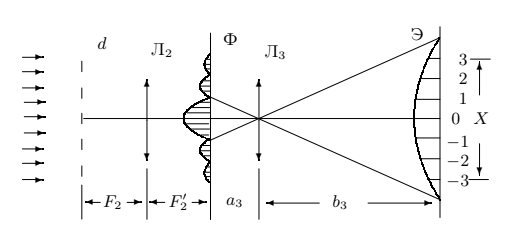
\includegraphics[width=15cm]{scheme_III.png}
            \caption{Схема лабораторной установки для наблюдения увеличенной дифракции на решетках}
            \label{fig:scheme_III}
        \end{figure}

        \itemЗная увеличение линзы ${Л_{3}}\left(\Gamma_{3}=b_{3} / a_{3}\right)$, можно рассчитать расстояние между максимумами $\Delta x$ в плоскости $\Phi$, а затем период сетки $d_{л}$ :
        $$
        \Delta x=\frac{\Delta X}{\Gamma_{3}}=\frac{\lambda}{d_{l}} F_{2}
        $$
        Занесем данные в таблицу \ref{table::with_lenses}:
\end{enumerate}


\begin{minipage}{0.5\textwidth}
    \begin{center}
    \begin{tabular}{|l|l|l|l|l|}
    \hline
    n & $X$, см & m  & $\Delta X$, мм & $d_c$, мкм \\ \hline
    1 & 14.5    & 4  & 36.3           & 21.8       \\ 
    2 & 14.7    & 6  & 24.5           & 32.3       \\ 
    3 & 14.5    & 12 & 12.1           & 65.5       \\ 
    4 & 12.0    & 20 & 6.00           & 132        \\ 
    5 & 12.5    & 24 & 4.79           & 165        \\ \hline
    \end{tabular}
    \captionof{table}{Дифракция без линз}
    \label{table::no_lenses}
    \end{center}
\end{minipage}
\begin{minipage}{0.5\textwidth}
    \begin{center}
    \begin{tabular}{|l|l|l|l|l|}
    \hline
    n & $X$, см & m  & $\Delta X$, см & $d_l$, мкм \\ \hline
    1 & 28.7    & 2  & 14.4           & 21.2       \\
    2 & 19.3    & 2  & 9.65           & 31.6       \\
    3 & 19.3    & 4  & 4.83           & 62.9       \\
    4 & 19.3    & 8  & 2.41           & 126        \\
    5 & 18.3    & 10 & 1.83           & 166        \\ \hline
    \end{tabular}
    \captionof{table}{Дифракция с линзами}
    \label{table::with_lenses}
    \end{center}
\end{minipage}
$$$$
Погрешность получившихся значений можно оценить как 
$$\sigma d_l \approx \sqrt{\left(\frac{\Delta F_2}{F_2}\right) + \left(\frac{\Delta X}{X}\right) + \left(\frac{\Delta L}{L}\right)} \approx 1\%$$

\section*{Пространственное преобразование спектров}

\begin{enumerate}
    \item Снова поставим тубус со щелью к окну лазера (рис. 4) и найдем на Экране резкое изображение щели с помощью линзы Л$_{2}\left(F_{2} = 11 \mathrm{~cm}\right) .$ В фокальной плоскости $\Phi$ линзы Л$_{2}$ поставим кассету с сетками, которые будут «рассекать» Фурье-образ щели - осуществлять пространственную фильтрацию. Подберем такую ширину входной щели $D$, чтобы на экране можно было наблюдать мультиплицированное изображение для всех сеток. Чем уже щель, тем шире её Фурье-образ и тем легче рассечь его сетками.
    
    \begin{figure}[h]
        \centering
        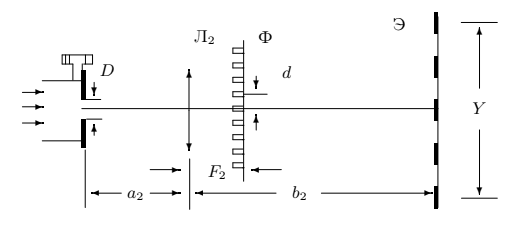
\includegraphics[width=15cm]{scheme_IV.png}
        \caption{Схема лабораторной установки рассечения Фурье-образа}
        \label{fig:scheme_IV}
    \end{figure}
    
    \newpage
    
    \item Снимем зависимость $Y$ (расстояние между удалёнными изображениями щели и и $k$ (число промежутков между изображениями) от $n$ (номер сетки) для фиксированной ширины входной щели. Данные занесем в Таблицу \ref{table::Fourier}.

    Запишем величину $D = ???$. Измерим расстояния $a_{2} = 11.8$ см и $b_{2} = 123$ см для расчёта увеличения $\Gamma_{2}$. Рассчитаем периоды $\Delta y$ «фиктивных» решёток, которые дали бы такую же периодичность на экране: $\Delta y=\Delta Y / \Gamma_{2}$, где $\Delta Y=Y / K .$

    Построим график $\Delta y=f\left(1 / d_{c}\right)$, где $d_{c}-$ периоды решёток, определённые по спектру:
        
    \begin{minipage}{0.5\textwidth}
        \centering
        \begin{tabular}{|l|l|l|l|l|}
        \hline
        n & k  & $Y$, см & $\Delta y$, мм & $1/d_l$, 1/ мм \\ \hline
        1 & 6  & 18.1    & 2.89           & 47.2           \\
        2 & 8  & 16.0    & 1.92           & 31.6           \\
        3 & 8  & 14.0    & 1.68           & 15.9           \\
        4 & 20 & 10.0    & 0.48           & 7.93           \\
        5 & 20 & 7.0     & 0.34           & 6.02           \\ \hline
        \end{tabular}
    \captionof{table}{Рассечение Фурье образа}
    \label{table::Fourier}
    \end{minipage}
    \begin{minipage}{0.5\textwidth}
        \begin{center}
            \begin{tikzpicture}[scale=1]
                \begin{axis}[
                    	axis lines = middle,
                    	xlabel = {$1/ d_l$, 1/мм},
                        ylabel = {$\Delta y$, мм},
                    	ylabel style={red, scale=1},
                        xlabel style={red, scale=1},
                    	title={Зависимость $\Delta y \left(1/d_l\right)$},
                    	table/col sep=semicolon,
                    ]
            	    \addplot +[blue, only marks] plot[
        			error bars/.cd,
        			x dir = both,
        			x fixed = 0.01,
        			y dir = both,
        			y fixed = 0,
        		    ] table[x=IDL, y=DDY]{fouri.csv};
		            \addplot[color=red, domain=5:50]{0.0616 * x - 0.0211};
            	\end{axis}
            \end{tikzpicture}
        \end{center}
    \end{minipage} 
    
    Зависимость должна быть линейной, поскольку
    $$
    \frac{\lambda}{\Delta y} F_{2}=d_{\mathrm{c}}
    $$
    
\end{enumerate}

\section{Вывод}

Мы пронаблюдали эффекты Фурье оптики такие как дифракция, рассечение изображения и фильтрация Фурье-компонент изображения.
Полученные нами результаты согласуются друг с другом:
\begin{enumerate}
    \item Двумя способами точно измерен момент открывания щели: 0.62 мм для метода геометрической оптики и 0.61 мм для дифракционного метода.
    \item Двумя способами измерены периоды решеток:
    \begin{table}[h]
        \centering
        \begin{tabular}{|l|l|l|l|l|l|}
        \hline
        $n$        & 1    & 2    & 3    & 4   & 5   \\ \hline
        $d_c$, мкм & 21.8 & 32.3 & 65.5 & 132 & 165 \\ \hline
        $d_l$, мкм & 21.2 & 31.6 & 62.9 & 126 & 166 \\ \hline
        \end{tabular}
    \end{table}
    \item Для фильтрации Фурье-образов отношения ширины щели при прямой фильтрации и под углом $45\deg$ получено отношение $\frac{0.26\text{мм}}{0.18\text{мм}} = 1.44 \approx \sqrt{2}$, как и предсказывает теория
\end{enumerate}


\end{document}
